% PSI Beamer presentation: exactly 20 physical pages, including the title.
% Results are frozen to the evidence in figure_sources.json/status_snapshot.json.
% The supplied PSI theme and assets are preserved without modification.
\PassOptionsToPackage{table}{xcolor}
\documentclass[aspectratio=169,10pt]{beamer}
\usetheme{PSI}
\usepackage{amsmath,amssymb}
\usefonttheme{professionalfonts}
\ifXeTeX
  \setsansfont{Liberation Sans}
\fi
\ifLuaTeX
  \setsansfont{Liberation Sans}
\fi
\graphicspath{{figures/}{psi-assets/}{./}}
\AtBeginSection[]{} % No automatic section pages: the deck stays at 20 pages.
\setbeameroption{hide notes}
\setbeamerfont{title}{size=\fontsize{25}{29}\selectfont,series=\bfseries}
\setbeamerfont{subtitle}{size=\fontsize{14}{18}\selectfont,series=\mdseries}
\renewcommand{\PSIfootername}{PSI \enspace | \enspace Pb--Bi--I deposition modelling}
\renewcommand{\PSIfootdate}{07.10.2026}
% Generated by prepare_figures.py; frozen until explicitly regenerated.
\newcommand{\SnapshotTime}{07 October 2026, 13:55 CEST}
\newcommand{\RunningCases}{16}
\newcommand{\QueuedCases}{47}
\newcommand{\CompletedCases}{1}
\newcommand{\FailedCases}{0}


\title{Iodine deposition\\in lead--bismuth systems}
\subtitle{Conservative CFD transport and thermochemical coupling\\Project review and validation programme}
\author{Jan Kren}
\institute{Villigen PSI}
\date{7 October 2026 \enspace | \enspace Working draft}
\psititlestyle{blue}

\newcommand{\PbI}{\ensuremath{\mathrm{PbI}_2}}
\newcommand{\BiI}{\ensuremath{\mathrm{BiI}_3}}
\newcommand{\sources}[1]{\par\vfill{\raggedright\fontsize{6.2}{7.5}\selectfont\color{PSIgray}#1\par}}
\newcommand{\takeaway}[1]{\par\vspace{0.2em}\begin{beamercolorbox}[sep=0.4em,wd=\linewidth]{block body}{\small\textbf{#1}}\end{beamercolorbox}}
\newcommand{\statuslabel}[2]{\textcolor{#1}{\textbf{#2}}}
\newcommand{\metric}[3]{\textcolor{PSIblue}{\fontsize{27}{31}\selectfont\textbf{#1}}\par\vspace{0.25em}\textbf{#2}\par{\small #3}}
\tikzset{process/.style={draw=PSIblue,fill=PSIblue!6,rounded corners=2pt,align=center,inner sep=7pt,font=\small},
  flow/.style={->,line width=1pt,draw=PSIblue}}

\begin{document}

% 01 --------------------------------------------------------------------
{\setbeamertemplate{footline}{}\setbeamertemplate{headline}{}
\begin{frame}[plain]
  \titlepage
  \note{This is a development review of the LESTO rhoFixedFlowFoam work. It presents completed numerical evidence and separates it from provisional experimental validation. All follow-up status counts are a dated snapshot.}
\end{frame}}

% 02 --------------------------------------------------------------------
\begin{frame}[t]{A working solver; physical validation is open}
  \begin{columns}[t,onlytextwidth]
    \begin{column}{0.30\textwidth}
      \metric{15}{Baseline cases passed}{60 s; 18,432 cells; 2 ms steps}
      \vspace{0.8em}
      \statuslabel{PSIblue}{IMPLEMENTED}\par
      \small Multi-species transport, equilibrium and conservative wall exchange.
    \end{column}
    \begin{column}{0.30\textwidth}
      \metric{5 / 5}{Q1 peak temperatures}{Within published uncertainty}
      \vspace{0.8em}
      \statuslabel{PSIred}{PROVISIONAL}\par
      \small Full profile agreement and predictive source chemistry remain unresolved.
    \end{column}
    \begin{column}{0.30\textwidth}
      \metric{64}{Follow-up cases}{Independent refinement and sensitivities}
      \vspace{0.8em}
      \statuslabel{PSIpurple}{IN PROGRESS}\par
      \small \RunningCases{} running; \QueuedCases{} queued.\par
      \small Snapshot: \SnapshotTime.
    \end{column}
  \end{columns}
  \takeaway{The next decision is whether the deposition profiles are numerically stable and which physical assumptions control them.}
  \sources{Evidence: run/034-liu2025/full\_analysis/analysis.json; status\_snapshot.json. Q1 uses prescribed iodide release.}
  \note{The five peak matches are from the available Q1 cases, not five independently predicted release mechanisms. M10a--d functionality is implemented; M10e scientific acceptance remains open. A numerical PASS reports execution and conservation gates.}
\end{frame}

% 03 --------------------------------------------------------------------
\begin{frame}[t]{Experiment: a source and a temperature gradient}
  \centering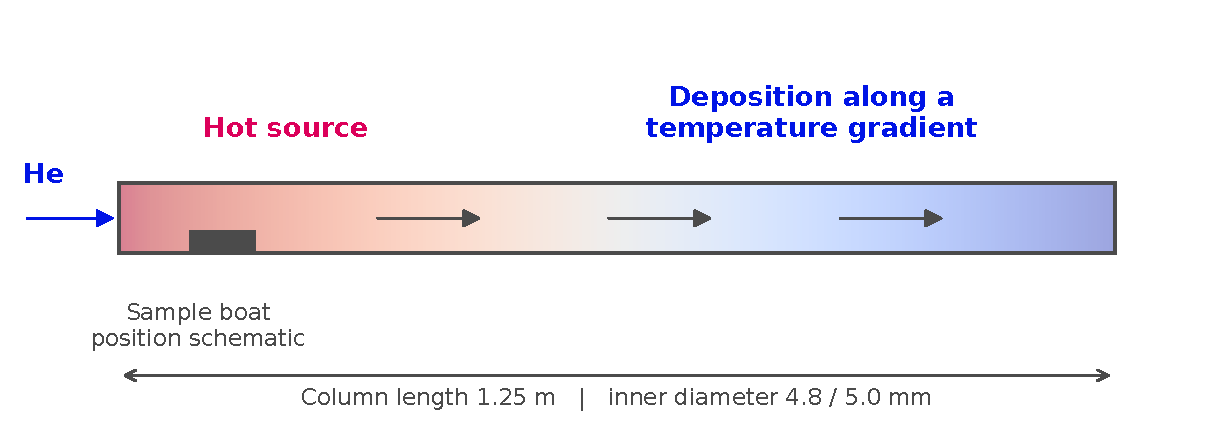
\includegraphics[width=0.96\linewidth,height=2.7cm,keepaspectratio]{experiment.pdf}
  \begin{columns}[t,onlytextwidth]
    \begin{column}{0.46\textwidth}
      \textbf{Published operating conditions}\par
      \small He flow: 100 mL/min for pure iodides; 45 mL/min for LBE--I.\par
      Three-hour exposure, then shutdown and cooling.
    \end{column}
    \begin{column}{0.48\textwidth}
      \textbf{Measured response}\par
      \small Axial iodine scan after cooling; deposit characterisation supports \PbI{} and \BiI{} identification.
    \end{column}
  \end{columns}
  \sources{Liu et al. (2025), DOI: 10.1007/s10967-025-10246-4, experimental section and Tables 2--5. Original schematic; not to scale. Current CFD: common 4.8 mm empty tube.}
  \note{Steel and silica inner diameters are respectively 4.8 and 5.0 mm in the paper. The CFD benchmark currently uses a common 4.8 mm diameter wedge, so the schematic must not imply a geometry-qualified silica simulation. Sample boat obstruction is omitted in the current empty-tube carrier.}
\end{frame}

% 04 --------------------------------------------------------------------
\begin{frame}[t]{Three published temperature profiles are available}
  \centering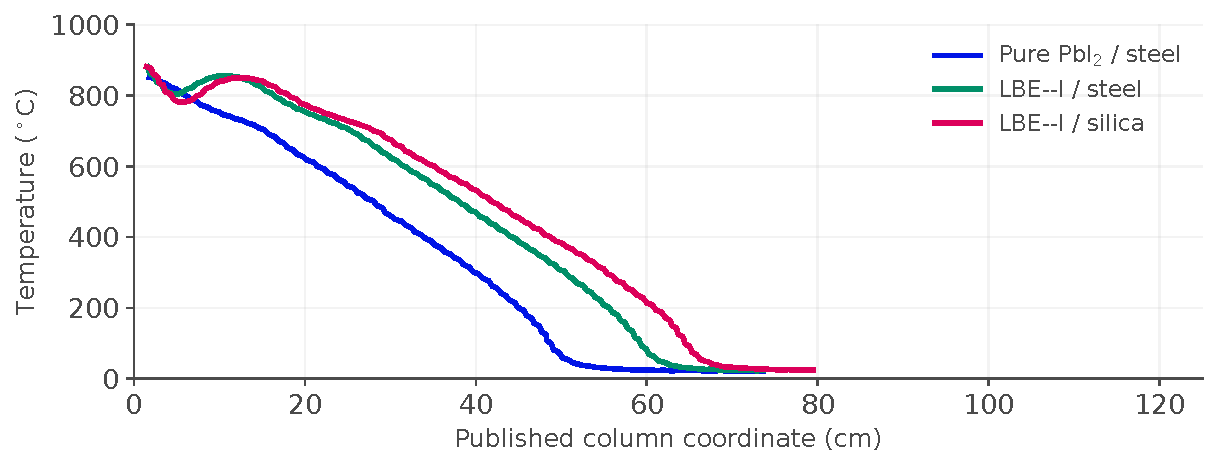
\includegraphics[width=0.96\linewidth,height=3.6cm,keepaspectratio]{temperatures.pdf}
  \takeaway{Temperature curves and iodine scans were digitised with their published coordinates; no alignment was fitted.}
  \sources{Liu et al. (2025), published figures; thermochemistry/benchmarks/liu2025/digitized/. BiI3\_SiO2\_800 lacks a plotted temperature profile and remains unrun.}
  \note{The available profiles are PbI2_SS, LBE-I_SS_II and LBE-I_SiO2_I. Digitisation is lower-information evidence than author-supplied numerical data. The silica curve and printed peak temperatures conflict; this is shown explicitly later.}
\end{frame}

% 05 --------------------------------------------------------------------
\begin{frame}[t]{A frozen carrier supports transient chemistry}
  \centering
  \begin{tikzpicture}
    \node[process,text width=2.1cm] (carrier) at (0,0) {Converged He flow\\$U,\,p,\,T,\,\rho,\,\phi$};
    \node[process,text width=2.1cm] (transport) at (3.1,0) {Species transport\\finite volumes};
    \node[process,text width=2.1cm] (chemistry) at (6.2,0) {Gas equilibrium\\Pb--Bi--I};
    \node[process,text width=2.1cm] (wall) at (9.3,0) {Wall exchange\\and deposit stores};
    \draw[flow] (carrier)--(transport);\draw[flow] (transport)--(chemistry);\draw[flow] (chemistry)--(wall);
    \node[process,text width=10cm] (ledger) at (4.65,-1.5) {Independent species, condensate and elemental accounts};
    \draw[flow] (transport.south)--(ledger.north -| transport.south);
    \draw[flow] (wall.south)--(ledger.north -| wall.south);
  \end{tikzpicture}
  \vspace{0.6em}
  \begin{itemize}
    \item Carrier momentum and temperature stay fixed during species transport.
    \item Current column matrix uses the gas kernel; GEMS frozen/local modes were qualified separately.
    \item Formation constants, source rates and solver inputs are fingerprinted.
  \end{itemize}
  \sources{rhoFixedFlowFoam implementation; phase-change-plan.md, sections 36.9--36.11 and 36.14--36.16. Diagram shows model components, not the exact operator sequence.}
  \note{The source is applied together with conservative transport and exchange; homogeneous respeciation follows gas transport and wall coproduct application. The diagram describes dependencies rather than promising a particular order. No energy equation or two-way feedback is solved in the current model.}
\end{frame}

% 06 --------------------------------------------------------------------
\begin{frame}[t]{Transport and phase change conserve material}
  \[
    \frac{\partial(\rho Y_i)}{\partial t}
    +\nabla\!\cdot(\rho\mathbf{u}Y_i)
    -\nabla\!\cdot(\rho D_i\nabla Y_i)=S_i
  \]
  \begin{columns}[t,onlytextwidth]
    \begin{column}{0.47\textwidth}
      \textbf{Transport}\par
      \begin{itemize}
        \item Frozen mass flux
        \item Diffusion and upwind advection
        \item Accounted source release
      \end{itemize}
    \end{column}
    \begin{column}{0.47\textwidth}
      \textbf{Wall exchange}\par
      \begin{itemize}
        \item Hertz--Knudsen--Schrage kinetics
        \item Half-cell diffusion resistance
        \item Bounded wall inventories
      \end{itemize}
    \end{column}
  \end{columns}
  \takeaway{Every transfer is booked consistently in gas, condensed material and Pb / Bi / I element balances.}
  \sources{applications/rhoFixedFlowFoam/readme.md; solvePairedGasSpecies.H and wall-channel accounting. Carrier He is separate from the nine reacting gases.}
  \note{The compact equation includes prescribed gas source terms; wall exchange is enforced through the coupled interface law rather than a fitted volumetric sink. S_i in this slide is schematic for sources. Conservation accounts include boundary transport and numerical corrections, which are also assessed independently.}
\end{frame}

% 07 --------------------------------------------------------------------
\begin{frame}[t]{Chemistry couples iodides and shared metal stores}
  \begin{columns}[t,onlytextwidth]
    \begin{column}{0.48\textwidth}
      \textbf{Nine transported reacting gases}\par
      \vspace{0.6em}
      \begin{tabular}{@{}lll@{}}
        $\mathrm{Pb}$ & $\mathrm{PbI}$ & $\mathrm{PbI}_2$\\[0.6em]
        $\mathrm{Bi}$ & $\mathrm{Bi}_2$ & $\mathrm{BiI}$\\[0.6em]
        $\mathrm{BiI}_3$ & $\mathrm{I}$ & $\mathrm{I}_2$
      \end{tabular}
      \vspace{0.8em}\par
      \small Helium supplies the carrier flow. Gas equilibrium preserves local elemental amounts.
    \end{column}
    \begin{column}{0.47\textwidth}
      \textbf{Condensed inventories}\par
      \begin{itemize}
        \item \PbI{} and \BiI{} deposits
        \item Shared Bi / Bi$_2$ store
        \item Pb metal store
      \end{itemize}
      \vspace{0.5em}
      \textbf{Reactive wall channel}\par
      \[
        3\,\mathrm{BiI(g)}\longrightarrow
        2\,\mathrm{Bi(s)}+\mathrm{BiI}_3\mathrm{(g)}
      \]
    \end{column}
  \end{columns}
  \takeaway{The deposited iodide split depends on source composition, gas speciation and surface reactions.}
  \sources{M10b gas kernel; M10d shared condensates and reactive wall channels. The displayed wall reaction is the implemented irreversible channel.}
  \note{Gas products are returned to the transport/respeciation system; wall Bi is deposited in the same physical store used by monomer and dimer exchange. Do not count that store twice in the element ledger. The channel is a model assumption, not a independently measured rate law for these surfaces.}
\end{frame}

% 08 --------------------------------------------------------------------
\begin{frame}[t]{Two source models answer different questions}
  \begin{columns}[t,onlytextwidth]
    \begin{column}{0.47\textwidth}
      \begin{block}{Q1: prescribed iodides}
        \small\raggedright\PbI{} and \BiI{} mean release rates are derived from published deposited amounts.\par\vspace{0.5em}
        \textbf{Purpose:} assess transport with a source constrained by the measured split.
      \end{block}
    \end{column}
    \begin{column}{0.47\textwidth}
      \begin{block}{Q2: atomic release}
        \small\raggedright I, Pb and Bi are supplied; gas chemistry forms iodides. Metal supply is a prescribed saturation fraction.\par\vspace{0.5em}
        \textbf{Purpose:} test source-conditioned predictions of the split.
      \end{block}
    \end{column}
  \end{columns}
  \takeaway{The 60 s CFD window retains the three-hour mean release rate: it supplies 1/180 of the assumed three-hour inventory.}
  \sources{run/034-liu2025 case manifests; Q1/Q2 source definitions in cases.py. The 5-degree wedge contains 1/72 of the full-column supply.}
  \note{Q1 split agreement is partly imposed by the source and must not be presented as independent validation of the release chemistry. The 60 s case does not compress a three-hour release into one minute. Q2 saturation is a provisional source parameter; neither source reconstructs an experimental release time series.}
\end{frame}

% 09 --------------------------------------------------------------------
\begin{frame}[t]{Verification covers equilibrium and conservation}
  \begin{columns}[t,onlytextwidth]
    \begin{column}{0.30\textwidth}
      \textbf{References}\par
      \begin{itemize}\small
        \item Wall closed forms
        \item Equilibrium oracle
        \item Plug-flow onsets
      \end{itemize}
    \end{column}
    \begin{column}{0.30\textwidth}
      \textbf{Robustness}\par
      \begin{itemize}\small
        \item Strong binding
        \item 600,000 stress inputs
        \item Guarded fallback
      \end{itemize}
    \end{column}
    \begin{column}{0.30\textwidth}
      \textbf{Consistency}\par
      \begin{itemize}\small
        \item Serial / four ranks
        \item Binary restarts
        \item Element ledgers
      \end{itemize}
    \end{column}
  \end{columns}
  \vspace{0.4em}
  \begin{block}{Follow-up launch checks}
    \small 64 / 64 native ten-step smoke checks passed; 9 carrier audits passed; 19 Python checks passed.
  \end{block}
  \sources{phase-change-plan.md, sections 36.9--36.16; run/034-liu2025/followup\_launch.json. These are targeted checks; no new aggregate Alltest or v2606 qualification is claimed.}
  \note{The 600,000-input equilibrium stress test used constants representative of the previously failed cells and had zero convergence or balance failures. The core kernel repair and targeted checks are documented. Smoke checks ensure the new configurations execute; they do not demonstrate full-window convergence or physical agreement.}
\end{frame}

% 10 --------------------------------------------------------------------
\begin{frame}[t]{All 15 available baseline cases finished}
  \psitablecolors{PSIblue}
  \begin{tabular}{@{}p{0.37\linewidth}p{0.19\linewidth}p{0.29\linewidth}@{}}
    \rowcolor{PSIblue}\psihead{Experiment} & \psihead{Cases} & \psihead{Source / thermodynamics}\\
    Pure \PbI{} / steel & 1 & Q1 / baseline\\
    LBE--I / steel & 7 & Q1 + six Q2 variants\\
    LBE--I / silica & 7 & Q1 + six Q2 variants\\
  \end{tabular}
  \vspace{0.8em}
  \begin{columns}[t,onlytextwidth]
    \begin{column}{0.30\textwidth}\textcolor{PSIblue}{\Large\textbf{$8.63\times10^{-16}$}}\par\small Maximum accounted element closure\end{column}
    \begin{column}{0.30\textwidth}\textcolor{PSIblue}{\Large\textbf{$5.98\times10^{-13}$}}\par\small Maximum raw material residue / supply\end{column}
    \begin{column}{0.30\textwidth}\textcolor{PSIblue}{\Large\textbf{0}}\par\small Gas-equilibrium solver failures\end{column}
  \end{columns}
  \takeaway{18,432 cells \enspace | \enspace 60 s \enspace | \enspace 2 ms \enspace | \enspace 15 PASS / 0 FAIL / 1 missing-profile NOTRUN}
  \sources{full\_analysis/analysis.json and independent material audits. BiI3\_SiO2\_800 is the unavailable case. Numerical PASS does not establish experimental validation.}
  \note{Each LBE experiment has a Q1 case and six Q2 cases: three saturation levels times two BiI thermodynamic variants. Raw residue is computed from actual material inventories and transport before numerical corrections. Accounted closure uses the conserved reference specified by the ledger.}
\end{frame}

% 11 --------------------------------------------------------------------
\begin{frame}[t]{Five Q1 peak temperatures match uncertainty bands}
  \centering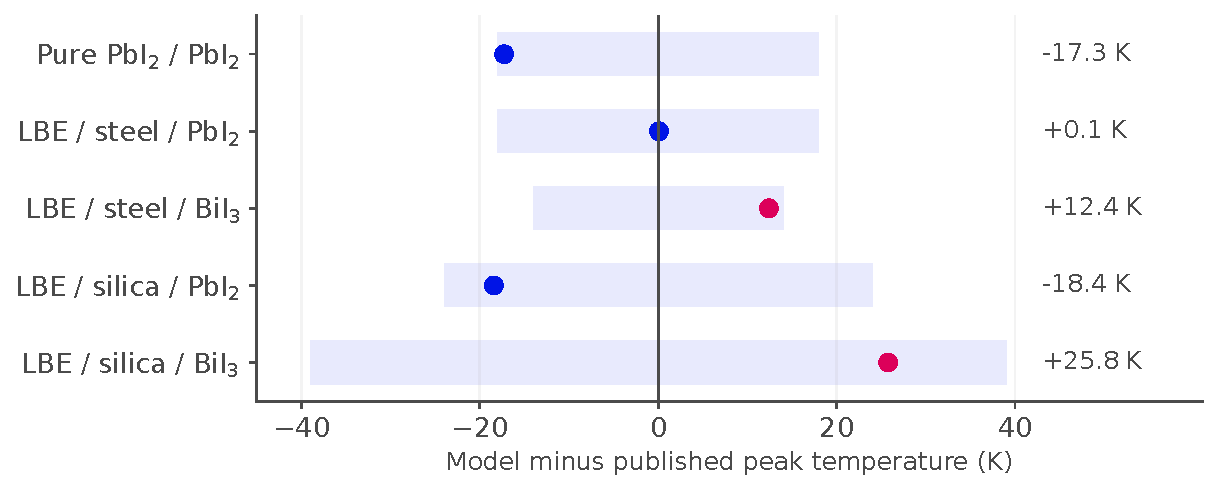
\includegraphics[width=0.97\linewidth,height=3.6cm,keepaspectratio]{peak_errors.pdf}
  \takeaway{Temperature agreement is encouraging; spatial profiles and source-conditioned species splits require separate assessment.}
  \sources{Liu et al. (2025), published deposition temperatures and uncertainties; full\_analysis/q1\_peaks.csv. Shaded bands show the published uncertainty around zero error.}
  \note{The plot is limited to the five available Q1 condensate peaks. The silica uncertainties are broad enough to contain temperature errors of about -18 and +26 K despite the 4--5 cm spatial mismatch. This is why peak-temperature agreement alone is insufficient.}
\end{frame}

% 12 --------------------------------------------------------------------
\begin{frame}[t]{Steel profiles reveal shape and split differences}
  \centering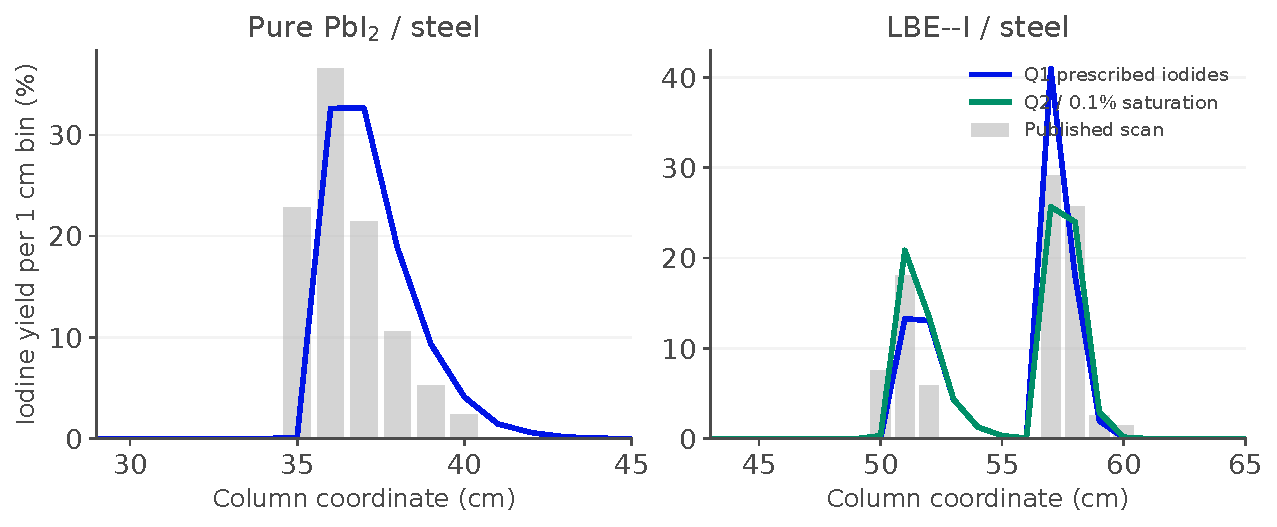
\includegraphics[width=0.98\linewidth,height=3.8cm,keepaspectratio]{steel_profiles.pdf}
  \small Steel Q2 at 0.1\% saturation: \BiI{} iodide-iodine share \textbf{56.47\%}, compared with \textbf{65.63\%} in the paper.
  \takeaway{The lowest tested steel profile error is still 36.80 percentage points in summed binwise absolute difference.}
  \sources{Digitised published scan heights retained; full\_analysis/case\_metrics.csv and saved iodine-comparison.csv. The LBE experimental scan includes KI; the model omits K chemistry.}
  \note{The error is the sum of absolute differences in per-bin percentage yield; it is not a 36.8\% relative scalar error. It is the lowest within the tested steel scenarios, not an optimised physical model. Model curves retain the same normalisation convention as the baseline analysis.}
\end{frame}

% 13 --------------------------------------------------------------------
\begin{frame}[t]{Silica deposition positions differ by 4--5 cm}
  \centering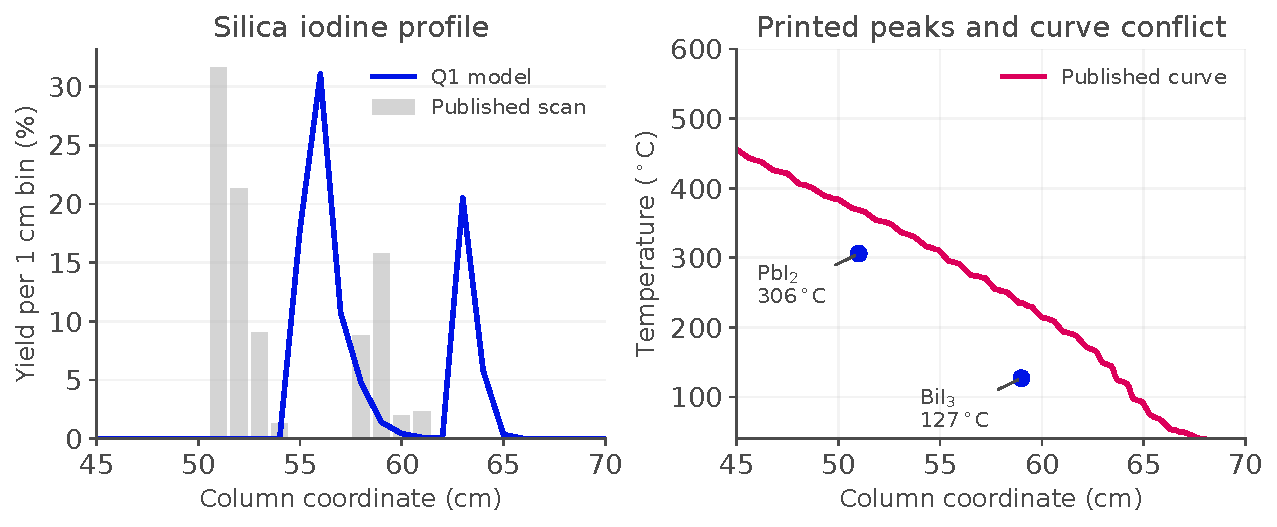
\includegraphics[width=0.98\linewidth,height=3.8cm,keepaspectratio]{silica_discrepancy.pdf}
  \begin{columns}[t,onlytextwidth]
    \begin{column}{0.46\textwidth}\small Q1 model / scan overlap is only about \textbf{7\%} after secondary normalisation over the common scan.\end{column}
    \begin{column}{0.48\textwidth}\small The printed peak temperatures conflict with the published curve at the scan maxima.\end{column}
  \end{columns}
  \sources{Liu et al. (2025), Figure 7 and printed peak temperatures; full\_analysis/silica\_figure\_diagnostics and case metrics. No coordinate correction applied in these plots.}
  \note{The model PbI2 and BiI3 peaks are respectively near 56 and 63 cm; published scan maxima are near 51 and 59 cm. Separate curve/label alignment hypotheses imply shifts about 4.10 and 4.65 cm, so the paper does not establish a unique correction. The ongoing shifted-curve cases are hypotheses.}
\end{frame}

% 14 --------------------------------------------------------------------
\begin{frame}[t]{BiI data and source loading can reverse the split}
  \centering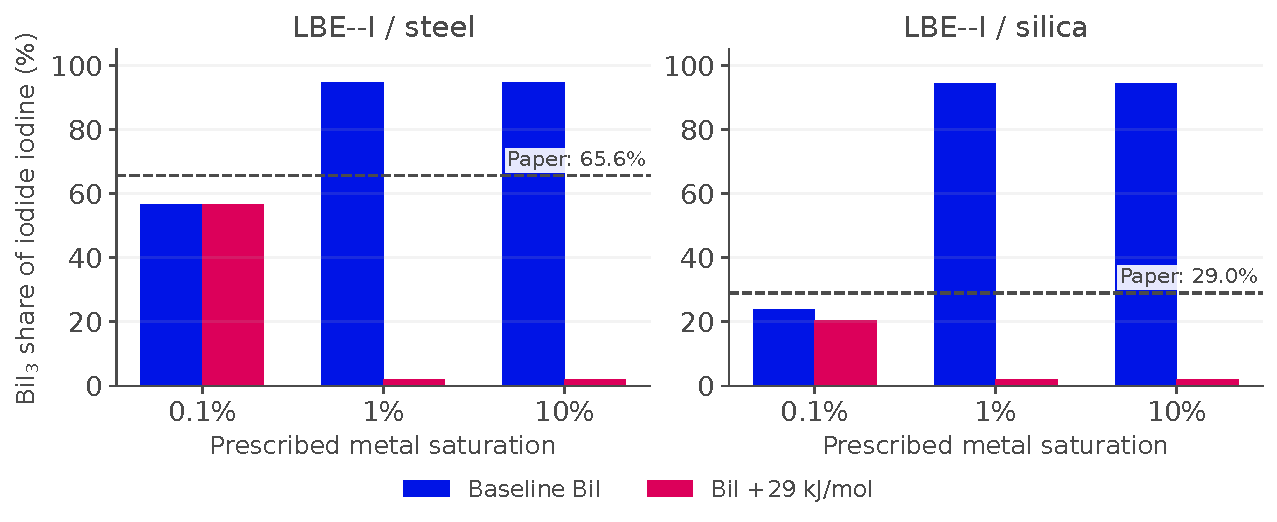
\includegraphics[width=0.98\linewidth,height=4.0cm,keepaspectratio]{thermodynamic_sensitivity.pdf}
  \takeaway{At 1\% metal saturation, the baseline and shifted BiI scenarios give roughly 94.5\% and 2\% \BiI{} shares.}
  \sources{full\_analysis/thermodynamic\_sensitivity.csv. Share = iodine in BiI3 / iodine in (PbI2 + BiI3). The +29 kJ/mol BiI shift is a surrogate sensitivity, not a second measured thermodynamic record.}
  \note{The two scenarios differ in BiI Gibbs formation energy consistently across formation, vapour-pressure and reaction tables. Large split differences show strong input sensitivity. The measured iodine split does not uniquely select thermodynamic data because the metal source is also unqualified. Dashed lines show the published iodide-only share.}
\end{frame}

% 15 --------------------------------------------------------------------
\begin{frame}[t]{Earlier refinement changed several factors together}
  \centering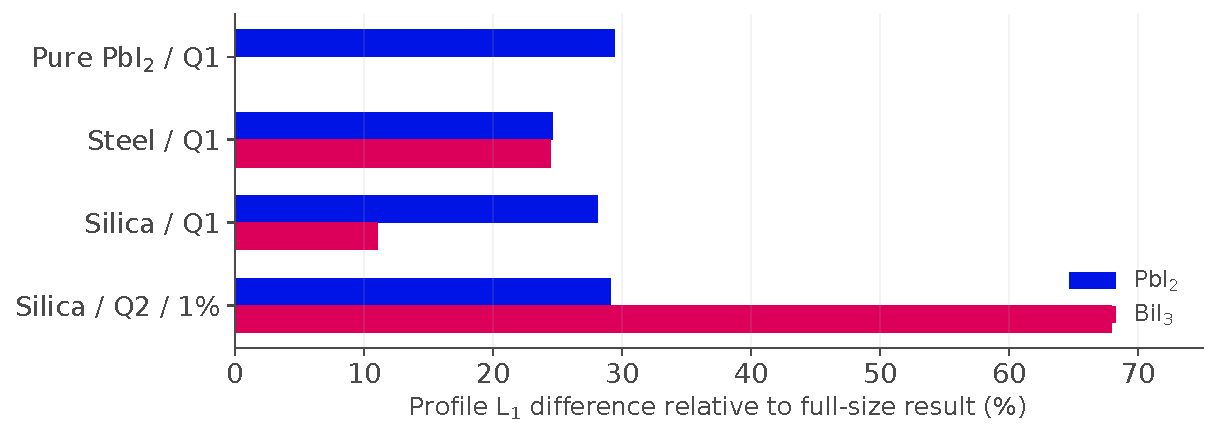
\includegraphics[width=0.95\linewidth,height=3.1cm,keepaspectratio]{mixed_refinement.pdf}
  \small Previous comparison: 2,048 $\rightarrow$ 18,432 cells; 20 $\rightarrow$ 2 ms; solver revision also changed.
  \takeaway{Profile changes reach 67.95\% L$_1$. First-order upwind numerical diffusion is comparable to the prescribed physical diffusion.}
  \sources{full\_analysis/combined\_refinement.csv; transport-scale estimates in analysis.json. This mixed comparison does not establish independent mesh or time convergence.}
  \note{Examples are shown rather than all 29 condensate comparisons. The 67.95\% maximum is BiI3 in the silica Q2 baseline at 1\% saturation. Total deposited amounts can change little while profile shapes change significantly. The numerical-diffusion estimate is a diagnostic, not a measured diffusivity.}
\end{frame}

% 16 --------------------------------------------------------------------
\begin{frame}[t]{Independent spatial and temporal refinement is running}
  \textbf{Fixed 2 ms time step: three meshes}\par\vspace{0.5em}
  \begin{columns}[t,onlytextwidth]
    \begin{column}{0.30\textwidth}\metric{8,192}{Coarse}{256 $\times$ 32 cells}\end{column}
    \begin{column}{0.30\textwidth}\metric{18,432}{Baseline}{384 $\times$ 48 cells}\end{column}
    \begin{column}{0.30\textwidth}\metric{41,472}{Fine}{576 $\times$ 72 cells}\end{column}
  \end{columns}
  \vspace{0.1em}
  \textbf{Fixed 18,432-cell mesh: 2 ms versus 1 ms}\par
  \small Four cases: pure \PbI{}, low/high metal loading and shifted BiI data.
  \begin{block}{Outputs used to decide adequacy}
    \small Profile L$_1$, centroid, amount and split; conditional three-grid estimates.
  \end{block}
  \sources{64-case study manifest; twelve new numerical cases. Uniform grid ratio 1.5 in each direction. Existing full-size results supply the medium grid / 2 ms reference.}
  \note{Three grids are not automatic proof of an asymptotic regime. The analysis declines to report an order or GCI for oscillatory, nondecreasing or roundoff-dominated scalar sequences. Mesh and temporal studies use the same private solver and retain original source rates and thermodynamic tables.}
\end{frame}

% 17 --------------------------------------------------------------------
\begin{frame}[t]{The 64-case study exposes provisional assumptions}
  \begin{columns}[t,onlytextwidth]
    \begin{column}{0.64\textwidth}
      \footnotesize\psitablecolors{PSIblue}\renewcommand{\arraystretch}{1.08}
      \begin{tabular}[t]{@{}p{0.48\linewidth}p{0.10\linewidth}p{0.30\linewidth}@{}}
        \rowcolor{PSIblue}\psihead{Study} & \psihead{N} & \psihead{Variation}\\
        Independent refinement & 12 & Mesh / time step\\
        Species diffusion & 12 & $0.5D$, $2D$, PbI$_2$--He\\
        Iodide accommodation & 8 & $\alpha=0.1,\ 0.01$\\
        Source position & 8 & $\pm15$ mm\\
        Source loading & 12 & Loading bracket\\
        Flow reference & 4 & $0\,^{\circ}\mathrm{C}$ alternative\\
        Silica alignment & 4 & Two hypotheses\\
        Isothermal flow stop & 4 & Restart 60--80 s\\
      \end{tabular}
    \end{column}
    \begin{column}{0.31\textwidth}
      \textbf{Frozen execution snapshot}\par\vspace{0.5em}
      \textcolor{PSIblue}{\Large\RunningCases{}} running\par
      \textcolor{PSIpurple}{\Large\QueuedCases{}} queued\par
      \textcolor{PSIgreen!60!black}{\Large\CompletedCases{}} full cases passed\par
      \textcolor{PSIred}{\Large\FailedCases{}} failed\par
      \vspace{0.7em}\footnotesize\SnapshotTime\par
      \vspace{0.7em}Up to 16 concurrent serial jobs; report generated after completion.
    \end{column}
  \end{columns}
  \sources{followup\_study.py; followup\_launch.json; dated status snapshot. Accommodation applies to iodide pairs; the empty-tube carrier still omits boat obstruction. No experimental parameter was fitted.}
  \note{The source loading values added between 0.1 and 1\% are 0.2, 0.316 and 0.562\%. Only PbI2 gets the species-specific He diffusivity model; other gases retain provisional coefficients. The 0-degree reference follows nominal manufacturer convention, not a confirmed calibration of the experimental controller. Counts are deliberately frozen for this draft.}
\end{frame}

% 18 --------------------------------------------------------------------
\begin{frame}[t]{Exposure duration and cooling need separate evidence}
  \begin{columns}[t,onlytextwidth]
    \begin{column}{0.47\textwidth}
      \begin{block}{Analytical duration}
        \small\raggedright Continue 50--60 s wall rates to 10,800 s.\par\vspace{0.5em}
        Assumes steady supply and deposition rates.\par\vspace{0.5em}
        Conditional gas iodine inventory: \textbf{0.010--0.0485\%} of three-hour supply.
      \end{block}
    \end{column}
    \begin{column}{0.47\textwidth}
      \begin{block}{Isothermal flow-stop CFD}
        \small\raggedright Restart at 60 s; stop source and carrier flow; advance to 80 s.\par\vspace{0.5em}
        Closed inventory; fixed temperature.\par\vspace{0.5em}
        Tests redistribution after flow stops.
      \end{block}
    \end{column}
  \end{columns}
  \takeaway{Experimental cooling could redistribute existing wall deposits. The paper supplies no measured temperature-versus-time history.}
  \sources{physical\_input\_audit/duration\_projection.csv (44 conditional profiles); shutdown case manifests; Liu experimental protocol. Neither study reconstructs the actual three-hour exposure plus cooling.}
  \note{The residual gas fraction uses the inventory at 60 s divided by a hypothetical three-hour steady iodine supply. It is not a bound on re-evaporation or redistribution of wall deposits during cooling. Analytical duration projections are not three-hour native CFD simulations. The fixed-temperature closed-end shutdown is a deliberately limited sensitivity experiment.}
\end{frame}

% 19 --------------------------------------------------------------------
\begin{frame}[t]{Decisions after the refinement study}
  \psitablecolors{PSIblue}
  \footnotesize\renewcommand{\arraystretch}{1.10}
  \begin{tabular}{@{}p{0.27\linewidth}p{0.34\linewidth}p{0.28\linewidth}@{}}
    \rowcolor{PSIblue}\psihead{Evidence} & \psihead{Decision} & \psihead{Remaining work}\\
    Mesh / time profiles & Select an adequate discretisation & Further refinement if needed\\
    Input sensitivities & Identify robust and source-sensitive predictions & Qualify thermodynamic / surface data\\
    Silica hypotheses & Assess effect of coordinate discrepancy & Confirm experimental temperature input\\
    Flow-stop / duration & Bound stated idealised effects & Obtain cooling and release evidence\\
    Completed scientific analysis & Define defensible manuscript claims & Final regression, archive, co-author review\\
  \end{tabular}
  \vspace{0.7em}
  \takeaway{The supplied paper supports a reproducible modelling and sensitivity study; stronger predictive claims require better-constrained inputs.}
  \sources{Physical input audit and M10e scientific acceptance criteria. Missing BiI3\_SiO2\_800 profile remains explicit. Broader M6/M8 comparison and validation requirements require separate reconciliation.}
  \note{No automatic acceptance is inferred when jobs finish. Convergence must be assessed for the physical quantities used in the claims. A follow-up can quantify sensitivity without identifying the true release history or wall kinetics. The manuscript is still a skeleton and will need final methods/results text and co-author review.}
\end{frame}

% 20 --------------------------------------------------------------------
\begin{frame}[t]{Conservative model; validation remains open}
  \begin{enumerate}
    \item \textbf{Implemented:} conservative transport, equilibrium and wall chemistry.
    \item \textbf{Verified numerically:} 15 baseline runs with tight element balances.
    \item \textbf{In progress:} profile convergence and physical-input sensitivity.
  \end{enumerate}
  \vspace{0.3em}
  \begin{block}{Next review}
    Review the 64-case results, select the numerical setup and define supported physical claims.
  \end{block}
  {\fontsize{7}{8.5}\selectfont
    \textbf{Primary references}\par
    Liu et al., \emph{J. Radioanal. Nucl. Chem.} 334 (2025), 5201--5216.\quad
    \href{https://doi.org/10.1007/s10967-025-10246-4}{doi:10.1007/s10967-025-10246-4}\par
    Lobresco et al., \emph{Nucl. Eng. Des.} 459 (2026), 115201.\quad
    \href{https://doi.org/10.1016/j.nucengdes.2026.115201}{doi:10.1016/j.nucengdes.2026.115201}\par
    \textbf{Project evidence:} baseline analysis, physical-input audit and follow-up launch record,\quad
    \href{https://github.com/JanKren/LESTO/tree/phase-change-rebased}{JanKren/LESTO}, study commit \texttt{361f02d}.
  }
  \note{The contribution is the reproducible implementation and an honest assessment of what the available experiments can constrain. The current deck is a first draft prepared while the refinement queue is active. Update dated status and result slides only after analysing completed follow-up evidence.}
\end{frame}

\end{document}
